\documentclass[10pt,twocolumn,letterpaper]{article}

\usepackage[pagenumbers]{cvpr}
\usepackage{graphicx}
\usepackage{booktabs}
\usepackage{amsmath}
\usepackage{multirow}
\usepackage{xcolor}
\usepackage{microtype}
\usepackage{caption}
\captionsetup{font=small}
\setlength{\abovecaptionskip}{4pt}
\setlength{\textfloatsep}{8pt}
\setlength{\tabcolsep}{4pt}

\definecolor{cvprblue}{rgb}{0.21,0.49,0.74}
\usepackage[breaklinks,colorlinks,allcolors=cvprblue]{hyperref}

\graphicspath{{figures/}}
\newcommand{\repourl}{\url{https://github.com/dishant1901-prog/ml_assignment_3_}}
\newcommand{\commit}{\texttt{cc5ae8bcd0c519739ad2c4854a536229ee90ee8e}}
\newcommand{\shortcommit}{\texttt{cc5ae8b}}

\def\confName{CVPR}
\def\confYear{2026}

\title{MLPs, CNNs, Autoencoders, SVMs and Clustering on CIFAR-10:\\
what the comparisons actually show}

\author{Dishant Kaushik\\
Roll number: M24MA2003\\
{\small Code: \repourl}\\
{\small Final commit: \commit}
}

\begin{document}
\maketitle

\begin{abstract}
We study four questions on CIFAR-10~\cite{krizhevsky2009cifar} with controlled comparisons rather than
leaderboard numbers. A fully connected network fits the training set but generalises poorly; a CNN with the
same parameter count and training budget gains 32 test points, while four times more MLP parameters gain 1.4.
Training on partly random labels shows that the MLP learns transferable structure in the first few epochs
and memorises afterwards. A fixed pixel permutation leaves the MLP unchanged but costs the CNN most of its
advantage, and shuffling image patches separates local evidence from global layout. For autoencoders,
reconstruction error and class information only agree roughly, and denoising recovers part, not all, of what a
fixed classifier needs. Finally an SVM and a clustering of the same autoencoder code are compared class pair by
class pair. All numbers quoted as final results are test-set numbers obtained after every choice was fixed on
validation data.
\end{abstract}

\section{Common setup}
\label{sec:setup}
\textbf{Data and split.} Images come from the CIFAR-10 parquet release \texttt{uoft-cs/cifar10} (revision
\texttt{0b27149}); it holds the same images as the official batches (identical channel statistics, test set in
the official order) but stores the training images in a different order, to which the saved split indices
refer. The 50{,}000 training images were split once into a stratified 45{,}000 /
5{,}000 train/validation split (4{,}500/500 per class) with seed \texttt{242003}, the digits of the roll number
M24MA2003 in order (\texttt{common/split\_seed242003.npz}). Every question loads this file. Inputs are normalised
per channel with the mean and standard deviation of the 45k training split. The validation split is used for
every model, architecture and hyper-parameter choice; the official 10k test set is evaluated only after the
choices are fixed, once per selected model.

\textbf{Training protocol (shared by Q1 and Q2).} 40 epochs, batch 128, SGD with Nesterov momentum 0.9, weight
decay $5\!\times\!10^{-4}$, OneCycle schedule (15\% warm-up), seed 242003. The peak learning rate is chosen per
model from $\{0.01, 0.03, 0.1, 0.3, 1.0\}$ by final-epoch validation accuracy. The grid started as
$\{0.01,\dots,0.1\}$ and was widened twice because a model was selected at its upper edge; every model was then
run on the full five-value grid, so tuning effort is identical. Train accuracy in all curves is measured in
evaluation mode on the un-augmented training images. Each configuration is run with one seed, so differences of
one to two points should not be over-read. Implementation: PyTorch~\cite{paszke2019pytorch} and
scikit-learn~\cite{pedregosa2011scikit}; no pretrained weights or external data.

\textbf{Reuse across questions.} Table~\ref{tab:reuse} lists every model or result used outside the question
that introduced it.

\begin{table}[t]
\centering
\small
\resizebox{\columnwidth}{!}{%
\begin{tabular}{@{}lll@{}}
\toprule
Component & Introduced & Reused in \\
\midrule
Split, normalisation, training loop & Setup & all \\
MLP 3072-336-336-10 and CNN (Tab.~\ref{tab:q1a}) & Q1(a) & Q2(a)--(c) \\
Clean-condition Q2 results (no retraining) & Q1(a) & Q2(a) \\
Selected Q1(a) CNN as fixed classifier & Q1(a) & Q3(b) \\
Clean AE-1024 & Q3(a) & Q3(b),(c) \\
DAE-1024 encoder (frozen) as representation & Q3(b) & Q3(c), Q4 \\
\bottomrule
\end{tabular}}
\caption{Models and results reused across questions.}
\label{tab:reuse}
\end{table}

\section{Q1: Why does an MLP do badly on CIFAR-10?}
\label{sec:q1}

\subsection{(a) Missing spatial prior or missing capacity?}
\textbf{Hypothesis.} An MLP treats the $3\times32\times32$ input as an unordered vector of 3072 numbers. It has
no notion that neighbouring pixels belong together or that a pattern means the same thing wherever it appears,
so it must learn locality and shift invariance from 45k images. Our claim is that it cannot, and that it ends
up \emph{fitting} the training set without generalising. The competing explanation is that the MLP is simply
too small or too hard to optimise, i.e.\ it \emph{underfits}.

\textbf{Design.} The two explanations make different predictions. Under the capacity explanation the MLP has low
training accuracy and more parameters raise validation accuracy clearly. Under the spatial-prior explanation the
MLP reaches high training accuracy, extra width barely helps, and a network with the prior built in does much
better at the \emph{same} parameter count and training budget. Four models were trained
(Tab.~\ref{tab:q1a}): a base MLP, a CNN with the same number of parameters, an MLP with 4.25$\times$ the
parameters (capacity test), and the base MLP with random flips and 4-pixel crops, which gives some shift
invariance through the data instead of the architecture. Both networks use BatchNorm and ReLU so neither gets a
normalisation advantage. The CNN is six $3\times3$ convolutions (64, 64, 128, 128, 256, 256 channels; max
pooling after the second and fourth), global average pooling and one linear layer.

\textbf{Fairness.} Parameters are matched to 0.14\%, epochs, optimiser, schedule, batch size, seed and
learning-rate grid are identical, and the learning rate is chosen on validation for each model. What is not
matched is computation per step: the CNN reuses each filter at every position and therefore performs many
more multiply-adds per parameter. We regard this as part of what the spatial prior is, not as an extra
advantage, but note it.

\begin{table}[t]
\centering
\small
\begin{tabular}{@{}lrcccc@{}}
\toprule
Model & Params & lr & Train & Val & Test \\
\midrule
MLP 3072-336-336-10 & 1{,}150{,}474 & 0.3 & 0.971 & 0.578 & 0.573 \\
Wide MLP 3072-1152-1152-10 & 4{,}884{,}490 & 0.1 & 1.000 & 0.600 & 0.587 \\
MLP + flip/crop & 1{,}150{,}474 & 0.1 & 0.664 & 0.615 & 0.621 \\
CNN (6 conv + GAP + FC) & 1{,}148{,}874 & 0.3 & 1.000 & 0.900 & \textbf{0.897} \\
\bottomrule
\end{tabular}
\caption{Q1(a). Selected learning rate, final-epoch train/val accuracy and the single test evaluation.}
\label{tab:q1a}
\end{table}

\begin{figure*}[t]
\centering
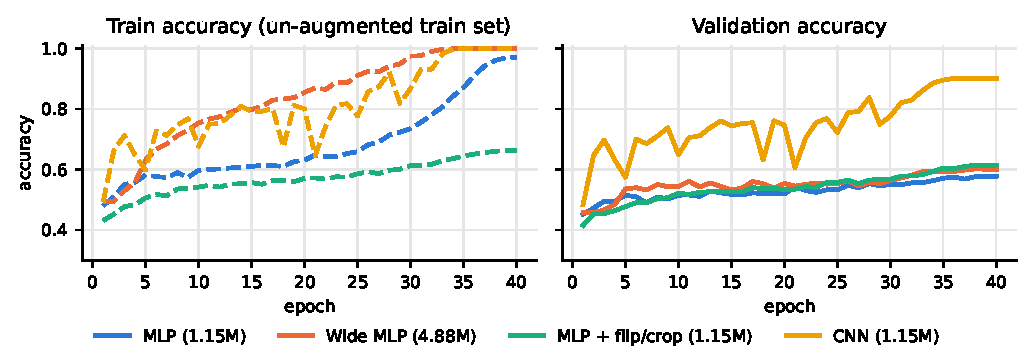
\includegraphics[width=\textwidth]{q1a_curves}
\caption{Q1(a) training curves of the selected runs. Train accuracy (left, dashed) and validation accuracy
(right). The MLPs reach (near) 100\% train accuracy while validation stays at 0.58--0.62.}
\label{fig:q1a}
\end{figure*}

\textbf{Result.} Capacity is not the bottleneck: the base MLP fits 97\% of the training set and the wide one
100\% (Fig.~\ref{fig:q1a}), yet 4.25$\times$ more parameters add only 1.4 test points. The train--val gap (0.39)
is the problem, not the training error. With the same parameter budget the CNN reaches 0.897 on test,
+32 points. Augmentation narrows the MLP's gap a lot (train 0.66 vs val 0.61) and adds 4.9 test points, so
small-shift invariance is part of the story, but the MLP stays 28 points behind. The evidence points to the
missing locality and weight sharing, which the MLP cannot learn from 45k images, rather than to underfitting.

\subsection{(b) Structure before memorisation}
\textbf{Setting.} 20\% of the 45k training labels were replaced by a different class chosen uniformly from the
other nine (seed 242003). Nothing in an image predicts its new label, so these examples cannot generalise and
can only be fitted by memorising them. The MLP was made large (3072-2048-2048-10, 10.5M parameters, about 230
per training image) and nothing discourages memorisation: no weight decay, no augmentation, constant learning
rate 0.002 (so changes in the curves are not caused by a schedule), 60 epochs. Two pilots (learning rate 0.01
and 0.002, one measurement per epoch) showed that everything happens in the first ~20 epochs, so the final runs
measure eight times per epoch. Runs with 0\% and 40\% relabelled examples serve as controls.

\textbf{Measurements across training.} At every measurement we record (i) accuracy on correctly labelled
training images, (ii) the fraction of relabelled images predicted as their \emph{wrong} training label
(memorisation), (iii) the fraction of relabelled images predicted as their \emph{true} class, and (iv) validation
accuracy (Fig.~\ref{fig:q1b}, Tab.~\ref{tab:q1b}).

\begin{figure*}[t]
\centering
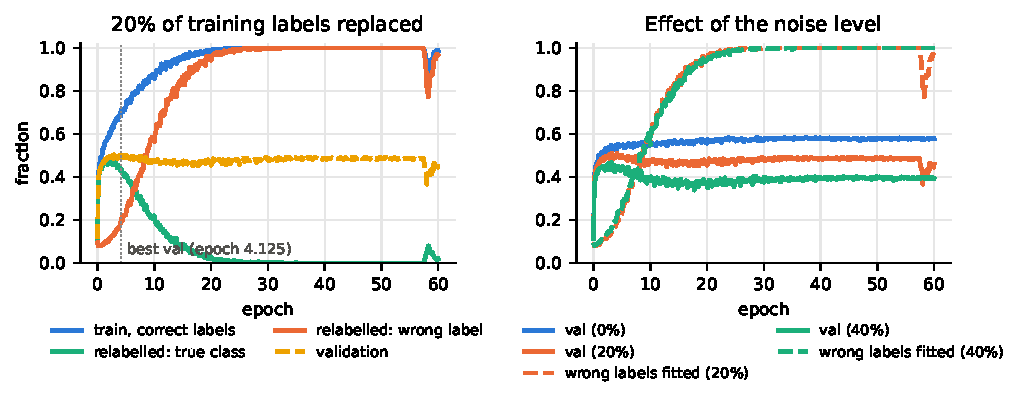
\includegraphics[width=\textwidth]{q1b_memorisation}
\caption{Q1(b). Left: 20\% relabelled. In the first epochs about 47\% of the relabelled training images are
predicted as their true class although the network is trained towards another label; validation peaks at
epoch 4.1, before the wrong labels overtake the true ones (epoch 6.5). Right: the same for 0/20/40\%. The dip
near epoch 58 is a single loss spike of the constant-lr run and is recovered within an epoch.}
\label{fig:q1b}
\end{figure*}

\begin{table}[t]
\centering
\small
\begin{tabular}{@{}rcccc@{}}
\toprule
Epoch & Train (correct) & Relab.$\to$true & Relab.$\to$wrong & Val \\
\midrule
1 & 0.534 & 0.461 & 0.086 & 0.471 \\
3 & 0.652 & 0.471 & 0.132 & 0.497 \\
4.1 & 0.710 & 0.439 & 0.190 & \textbf{0.512} \\
8 & 0.818 & 0.284 & 0.431 & 0.479 \\
15 & 0.952 & 0.088 & 0.837 & 0.459 \\
30 & 1.000 & 0.000 & 1.000 & 0.478 \\
\midrule
\multicolumn{5}{@{}l}{Test acc.\ (best-val checkpoint / final): 0\%: 0.565 / 0.564;} \\
\multicolumn{5}{@{}l}{20\%: 0.503 / 0.457;\quad 40\%: 0.459 / 0.395} \\
\bottomrule
\end{tabular}
\caption{Q1(b), 20\% relabelled. Bottom: test accuracy of the checkpoint with the best validation accuracy
(selected on validation) and of the final, memorising model.}
\label{tab:q1b}
\end{table}

\textbf{Interpretation.} Useful structure is learned first. In the first three epochs the network predicts the
\emph{true} class for 47\% of the relabelled images while being pushed towards a different label; it can only do
this with features that transfer across images, and validation accuracy rises at the same time. Memorisation
starts afterwards: the wrong-label fit grows from 0.13 (epoch 3) to 0.43 (epoch 8) and 1.00 (epoch 30), the
true-class fraction collapses, and validation drops from its peak of 0.512 at epoch 4.1. The peak comes before
the crossover at epoch 6.5. With clean labels, validation keeps improving until epoch 29 and does not fall, so
the drop in the noisy runs comes from fitting the wrong labels, not from long training as such; at 40\% noise the
peak and the crossover come earlier and the drop is larger. On test, early stopping on validation keeps 4.6
(20\%) and 6.3 (40\%) points that the memorising model loses, while with clean labels the two coincide. This
agrees with the ordering reported by Arpit~\etal~\cite{arpit2017closer} and with the observation that such
networks can fit random labels~\cite{zhang2017rethinking}.

\section{Q2: CNN versus MLP}
\label{sec:q2}

\subsection{(a) A fair comparison and a proposed reason}
\textbf{Fairness criterion (written down before any test number existed).} The two models are the Q1(a) MLP
(1{,}150{,}474 parameters) and CNN (1{,}148{,}874), reused from Q1. They are compared at matched parameter
count and matched training budget: the same 45k images, 40 epochs, optimiser, schedule, batch size, weight
decay, seed and BatchNorm/ReLU; the same learning-rate grid with selection on validation; and no augmentation
for either, because flips and crops assume an intact spatial layout and would not be the same treatment once the
pixels are permuted in (b). Computation per step is not matched (see Q1). Each model is tested once after
selection.

\textbf{Proposed reason (also stated beforehand).} The CNN's advantage comes from exploiting the local spatial
arrangement of pixels: neighbouring pixels are strongly correlated and the same local pattern can occur
anywhere, which local receptive fields and weight sharing~\cite{lecun1998gradient} use directly. The MLP has no
access to this arrangement.

\begin{table}[t]
\centering
\small
\begin{tabular}{@{}lcccc@{}}
\toprule
& \multicolumn{2}{c}{MLP (1{,}150{,}474)} & \multicolumn{2}{c}{CNN (1{,}148{,}874)} \\
\cmidrule(lr){2-3}\cmidrule(l){4-5}
Condition & lr & Test & lr & Test \\
\midrule
Clean (Q1(a) runs) & 0.3 & 0.573 & 0.3 & \textbf{0.897} \\
Pixel permutation & 0.3 & 0.576 & 0.3 & 0.561 \\
$16\times16$ patches shuffled & 0.3 & 0.403 & 0.3$^*$ & 0.815 \\
$8\times8$ patches shuffled & 1.0 & 0.324 & 0.3 & 0.705 \\
$4\times4$ patches shuffled & 1.0 & 0.276 & 0.3$^*$ & 0.602 \\
\bottomrule
\end{tabular}
\caption{Q2. Compared models with parameter counts and test accuracy under each condition (train and test use
the same transformation). $^*$CNN learning rate taken from the $8\times8$ validation result; all others chosen
on validation from the full grid.}
\label{tab:q2}
\end{table}

\begin{figure}[t]
\centering
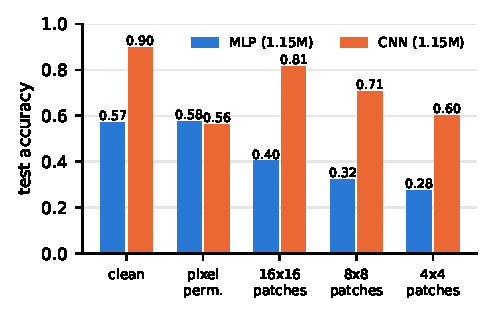
\includegraphics[width=\columnwidth]{q2_accuracy_by_condition}
\caption{Q2. Test accuracy of the MLP and CNN under the clean, permuted and patch-shuffled conditions.}
\label{fig:q2acc}
\end{figure}

\textbf{Result.} Under this criterion the CNN reaches 0.897 and the MLP 0.573 on test (Tab.~\ref{tab:q2}), a gap
of 32.4 points that can only come from how the same number of parameters is wired.

\subsection{(b) Same pixels, disturbed spatial structure}
\textbf{Transformation.} One fixed random permutation of the 1024 pixel positions (seed 242003), applied
identically to the three colour channels and to every training, validation and test image. Pixel values are
unchanged and the mapping is the same for every image, so all information is still present; only the
neighbourhood structure is gone. Both models were retrained from scratch with the same protocol and grid.

\textbf{Prediction (stated before running).} The MLP should not change beyond noise (about one point): a fixed
permutation of its inputs is equivalent to permuting the rows of its first weight matrix, so the function class
is identical and only the initialisation and batch order differ. The CNN should drop to roughly the MLP level or
below, since its $3\times3$ filters and pooling now combine pixels that are not neighbours. If the CNN kept most of
its advantage, the reason proposed in (a) would be wrong.

\textbf{Result.} Both predictions hold (Tab.~\ref{tab:q2}, Fig.~\ref{fig:q2acc}). The MLP moves from 0.573 to
0.576, within noise. The CNN falls from 0.897 to 0.561, slightly \emph{below} the permuted MLP, although every
pixel value is still available. Destroying neighbourhoods removes the CNN's entire advantage, which supports the
reason proposed in (a); with the arrangement gone, its local filters even work slightly against it.

\subsection{(c) Local evidence or global layout?}
Two explanations for what the CNN uses remain after (b): (A) \emph{local evidence}, i.e.\ textures, colours and
small parts within small windows (a ``bag of local features''~\cite{brendel2019bagnet}), or (B) the \emph{global
layout} of those parts, i.e.\ object shape and configuration. Both need intact neighbourhoods, so (b) cannot tell
them apart. We cut each image into a grid of $p\times p$ patches and put the patches back in a random order that
is different for every image (fixed seeds per split, the same procedure for train, validation and test). Inside a
patch everything is intact; between patches the arrangement is destroyed. If (A) holds, accuracy should stay high
once patches are big enough to contain a recognisable part; if (B) matters, it should drop strongly even for large
patches. We use $p=8$ as the main condition (both models, full learning-rate grid) and $p=4$ and $p=16$ as a
sweep (CNN learning rate taken from the $p=8$ validation result; MLP full grid). Errors and confidence are
analysed on test.

\begin{figure*}[t]
\centering
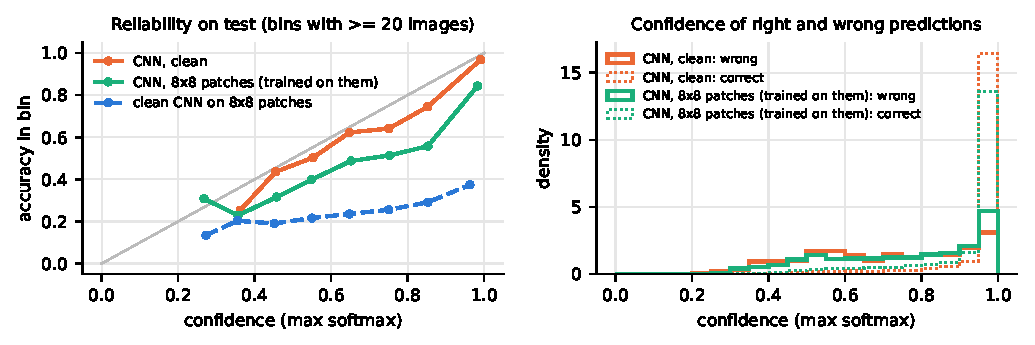
\includegraphics[width=\textwidth]{q2_confidence}
\caption{Q2(c), test set. Left: reliability of the clean CNN, the CNN trained and tested on $8\times8$ shuffles,
and the clean CNN tested on $8\times8$ shuffles. Right: confidence of correct (dotted) and wrong (solid)
predictions.}
\label{fig:q2conf}
\end{figure*}

\begin{table}[t]
\centering
\small
\begin{tabular}{@{}lccccc@{}}
\toprule
CNN, test & Acc. & Conf.\ right & Conf.\ wrong & Wrong $>0.9$ & ECE \\
\midrule
Clean & 0.897 & 0.956 & 0.710 & 25\% & 0.033 \\
$16\times16$ & 0.815 & 0.938 & 0.730 & 28\% & 0.085 \\
$8\times8$ & 0.705 & 0.919 & 0.753 & 34\% & 0.164 \\
$4\times4$ & 0.602 & 0.894 & 0.753 & 33\% & 0.236 \\
Clean model on $8\times8$ & 0.277 & 0.781 & 0.707 & 27\% & 0.450 \\
\bottomrule
\end{tabular}
\caption{Q2(c). Mean max-softmax confidence of right and wrong predictions, share of errors made with
confidence above 0.9, and expected calibration error (15 bins)~\cite{guo2017calibration}.}
\label{tab:q2conf}
\end{table}

\textbf{Accuracy.} Accuracy falls gradually as patches shrink: 0.897 (intact), 0.815 ($p=16$), 0.705 ($p=8$),
0.602 ($p=4$) and 0.561 for single pixels (the permutation of (b)). With $8\times8$ patches in a random order the
CNN keeps 79\% of its clean accuracy and stays 38 points above the MLP under the same shuffle, so local evidence
(A) carries most of its performance. The MLP collapses (0.573 to 0.324) because its weights are tied to absolute
positions. Layout (B) is not irrelevant: shuffling $8\times8$ patches still costs the CNN 19 points.

\textbf{Errors.} The loss is not uniform. Per-class recall drops most for cat ($-27$), deer ($-26$), bird
($-22$), horse ($-22$) and dog ($-21$) and least for ship ($-10$) and truck ($-14$). The confusions that grow are
between classes that share texture and colour and differ mainly in shape: dog$\to$cat 89$\to$178,
cat$\to$dog 76$\to$175, automobile$\to$truck 34$\to$108, deer$\to$frog 15$\to$93. Classes with distinctive
local context (water around ships, frog skin texture) survive.

\textbf{Confidence.} The clean CNN is well calibrated (ECE 0.033, Tab.~\ref{tab:q2conf}, Fig.~\ref{fig:q2conf}).
Without layout the CNN does not become uncertain: its confidence on \emph{wrong} predictions rises (0.710 to
0.753) and 34\% of its errors are made with more than 0.9 confidence. It decides confidently from local evidence
and is simply wrong more often, which is what a bag-of-local-features decision would do. As a side check, the
clean-trained CNN applied to $8\times8$-shuffled test images (not a train=test condition) drops to 0.277 at 0.73
mean confidence: trained on intact images it does use the layout it is given.

\textbf{Conclusion linking (a)--(c).} The CNN wins by 32 points at equal budget (a). Removing pixel
neighbourhoods removes the whole gain, so the gain comes from spatial arrangement (b). Of that arrangement, local
neighbourhoods carry most of the accuracy, and global layout contributes a smaller part concentrated in classes
that look alike locally (c).

\section{Q3: Autoencoders}
\label{sec:q3}

\subsection{(a) Bottleneck capacity}
The three convolutional autoencoders share everything except the bottleneck. The encoder is three stride-2
$4\times4$ convolutions (32, 64, 128 channels, BatchNorm, ReLU) down to $128\times4\times4$ followed by a linear
layer to a $d$-dimensional code; the decoder mirrors it with transposed convolutions. Only the two linear
layers change with $d \in \{16, 128, 1024\}$ (192$\times$, 24$\times$ and 3$\times$ compression of the 3072
input values). All three are trained identically without labels: AdamW (lr $10^{-3}$, weight decay
$10^{-5}$), OneCycle, 30 epochs, batch 256, MSE in the normalised input space, seed 242003. Working in the
normalised space lets reconstructions go straight into the Q1 classifier; errors are also reported in $[0,1]$
pixel units.

\begin{table}[t]
\centering
\small
\begin{tabular}{@{}rrcc@{}}
\toprule
$d$ & Params & Val MSE (norm.) & Val MSE (pixel) \\
\midrule
16 & 398{,}995 & 0.2633 & 0.01650 \\
128 & 857{,}859 & 0.0800 & 0.00502 \\
1024 & 4{,}528{,}771 & 0.0308 & \textbf{0.00194} \\
\bottomrule
\end{tabular}
\caption{Q3(a). Validation reconstruction error after 30 epochs. Selected: $d=1024$; its test MSE is 0.00194
(pixel), PSNR 27.1\,dB.}
\label{tab:q3a}
\end{table}

If reconstruction error is the only criterion there is no trade-off to make: validation error falls steadily
with $d$ (Tab.~\ref{tab:q3a}), so $d=1024$ is selected. Its test error (0.00194) equals its validation error,
so the choice did not overfit the validation split. It is still far from an identity map: fine texture and
sharp edges are smoothed (Fig.~\ref{fig:q3rec}, row 4).

\begin{figure}[t]
\centering
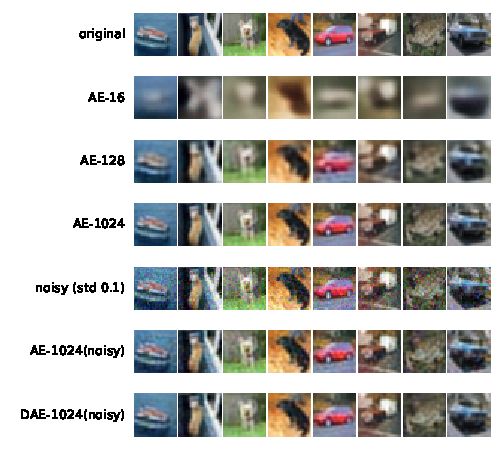
\includegraphics[width=\columnwidth]{q3_reconstructions}
\caption{Q3. Test images and their reconstructions by the three clean autoencoders, the noisy input
($\sigma=0.1$), and the clean AE and the DAE applied to the noisy input.}
\label{fig:q3rec}
\end{figure}

\subsection{(b) Does denoising recover what the classifier needs?}
\textbf{Corruption and protocol.} Additive Gaussian noise with standard deviation $\sigma=0.1$ in $[0,1]$ pixel
units, clipped to $[0,1]$. Reconstruction can reasonably help here because the noise is independent per pixel
while natural images are smooth and correlated (unlike occlusion or blur, which remove information that can only
be guessed). The denoising autoencoder (DAE)~\cite{vincent2008extracting} has the same architecture and
bottleneck as the selected clean AE and the same optimiser, schedule and epochs; its input is a noisy image
(noise redrawn every batch) and its target the clean image. No labels are used. The classifier is the selected
Q1(a) CNN (test accuracy 0.897), kept fixed. Test noise is drawn once with a fixed seed; we also report
$\sigma=0.05$ and $0.2$, and the classifier on reconstructions of \emph{clean} images as a control.

\begin{table}[t]
\centering
\small
\begin{tabular}{@{}lccc@{}}
\toprule
Classifier input & $\sigma=0.05$ & $\sigma=0.1$ (train) & $\sigma=0.2$ \\
\midrule
Noisy image & \textbf{0.655} & 0.280 & 0.115 \\
Clean AE (noisy) & 0.616 & \textbf{0.553} & 0.406 \\
DAE (noisy) & 0.548 & 0.524 & \textbf{0.422} \\
\midrule
\multicolumn{4}{@{}l}{Control, no noise: clean image 0.897; clean AE 0.646; DAE 0.553} \\
\multicolumn{4}{@{}l}{MSE to clean at $\sigma=0.1$: noisy 0.0093, AE 0.0032, DAE 0.0030} \\
\bottomrule
\end{tabular}
\caption{Q3(b). Test accuracy of the fixed Q1(a) CNN.}
\label{tab:q3b}
\end{table}

\textbf{Result.} At the trained noise level the DAE brings the classifier from 0.280 back to 0.524
(Tab.~\ref{tab:q3b}), so it recovers a large part of what the noise destroyed, but nowhere near the clean
0.897. The control rows explain why: a \emph{clean} image passed through the clean AE already drops to 0.646, and
through the DAE to 0.553. Both autoencoders keep layout and colour but remove texture and edges the CNN relies
on, so about 0.65 is a ceiling for reconstruct-then-classify with these models. Two further observations show
that pixel error is the wrong yardstick. The DAE's outputs are closer to the clean images in MSE than the clean
AE's (0.0030 vs 0.0032) yet give lower accuracy (0.524 vs 0.553): it smooths more aggressively, which lowers MSE
against noise and also removes texture. And the DAE is the best option only at the stronger noise $\sigma=0.2$;
at $\sigma=0.05$ the noisy image itself is better than either reconstruction. Our answer is therefore that
denoising recovers \emph{some} class information (+24 points) but not the information the classifier needs to
approach its clean accuracy, because the reconstruction step removes it. Part of the loss is a distribution
shift for a classifier trained on sharp images; retraining it on reconstructions would be a different experiment
and is excluded by the question.

\subsection{(c) Class information vs reconstruction quality}
The encoders are frozen and their bottleneck codes are probed in two ways: a multinomial logistic regression
(features standardised with train statistics, L2 weight in $\{10^{-5},\dots,10^{-1}\}$ chosen on validation) and
a cosine $k$-NN ($k\in\{1,\dots,100\}$ chosen on validation). Raw pixels are included as a reference.

\begin{table}[t]
\centering
\small
\begin{tabular}{@{}lccccc@{}}
\toprule
Code & Dim & MSE (px) & PSNR & Linear & $k$-NN \\
\midrule
AE-16 & 16 & 0.0165 & 17.8 & 0.331 & 0.422 \\
AE-128 & 128 & 0.0050 & 23.0 & 0.410 & 0.409 \\
AE-1024 & 1024 & \textbf{0.0019} & \textbf{27.1} & 0.532 & 0.485 \\
DAE-1024 & 1024 & 0.0024 & 26.1 & \textbf{0.550} & \textbf{0.490} \\
Raw pixels & 3072 & -- & -- & 0.415 & 0.426 \\
\bottomrule
\end{tabular}
\caption{Q3(c). Test reconstruction error of clean images and test accuracy of probes on frozen codes.}
\label{tab:q3c}
\end{table}

\begin{figure}[t]
\centering
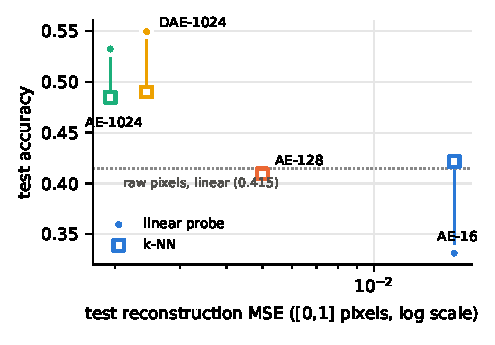
\includegraphics[width=0.9\columnwidth]{q3_recon_vs_probe}
\caption{Q3(c). Reconstruction error (log) against test accuracy of a linear probe (dots) and $k$-NN (squares)
on the frozen code. The two AE-128 markers overlap (0.410 / 0.409).}
\label{fig:q3c}
\end{figure}

Across the three clean autoencoders, better reconstruction goes with more linearly available class information
(0.331, 0.410, 0.532), so at a coarse level the two agree (Tab.~\ref{tab:q3c}, Fig.~\ref{fig:q3c}). They part
ways in two places. The DAE reconstructs clean images worse than AE-1024 but its code holds more class
information (0.550 vs 0.532 linear; the $k$-NN gap of 0.5 points is within single-seed noise). A plausible reason
is that removing noise forces the code to keep structure that is stable under small pixel changes, which is more
related to the class than exact pixel values. Second, under $k$-NN the 16-d code (0.422) beats the 128-d code
(0.409) despite three times the reconstruction error, while the linear probe ranks them the other way. Moreover,
AE-128 is no better than raw pixels at all. We conclude that the two quantities agree only roughly and that
reconstruction error is not a reliable proxy for how useful a representation is for classification.

\section{Q4 (bonus): SVMs and clustering on one fixed representation}
\label{sec:q4}

\textbf{Representation.} The 1024-d bottleneck code of the Q3(b) denoising autoencoder, frozen. Among the Q3
encoders it has the highest \emph{validation} linear-probe accuracy (0.553), so it is chosen without test
data; it was trained without labels, which keeps the clustering in (c) genuinely unsupervised. Codes are
standardised with the mean and standard deviation of the 45k training codes and never changed afterwards.
\textbf{Subset.} A kernel SVM on 45k$\times$1024 is slow (one RBF fit on 10k points takes 2--4 minutes), so a
stratified subset of 10{,}000 training images (1{,}000 per class, seed 242003) was drawn and saved
\emph{before any SVM was fitted}; every SVM uses it. Validation is the full 5k split and test the full 10k set.

\subsection{(a) Effect of C and the kernel}
We use scikit-learn's \texttt{SVC} (libsvm, one-vs-one)~\cite{cortes1995support,pedregosa2011scikit} with
$C\in\{10^{-3},\dots,10^{2}\}$ (six values, five orders of magnitude; $10^{-3}$ was added after the linear kernel
selected the lower edge of the first grid) and three kernels: linear, RBF ($\gamma=1/(d\,\mathrm{Var}(x))$) and
polynomial of degree 3 ($\gamma$ as for RBF, $c_0=1$). Table~\ref{tab:q4sweep} gives the full sweep and
Fig.~\ref{fig:q4sweep} the curves.

\begin{table}[t]
\centering
\small
\begin{tabular}{@{}l@{\hspace{3pt}}cccccc@{}}
\toprule
& \multicolumn{6}{c}{$C$} \\
\cmidrule(l){2-7}
Kernel / metric & $10^{-3}$ & $10^{-2}$ & $10^{-1}$ & $1$ & $10$ & $10^{2}$ \\
\midrule
Linear\hfill train & .573 & .681 & .832 & .954 & .997 & 1.00 \\
\hfill val & .456 & \textbf{.467} & .438 & .422 & .409 & .406 \\
\hfill SV & .905 & .853 & .823 & .807 & .801 & .799 \\
\midrule
RBF\hfill train & .324 & .324 & .477 & .841 & .998 & 1.00 \\
\hfill val & .295 & .295 & .405 & .512 & \textbf{.539} & .539 \\
\hfill SV & 1.00 & 1.00 & .989 & .953 & .965 & .964 \\
\midrule
Poly-3\hfill train & .359 & .489 & .753 & .974 & 1.00 & 1.00 \\
\hfill val & .340 & .429 & .509 & \textbf{.531} & .518 & .516 \\
\hfill SV & 1.00 & .988 & .942 & .928 & .921 & .920 \\
\bottomrule
\end{tabular}
\caption{Q4(a). Train accuracy (10k subset), validation accuracy and fraction of training points that are
support vectors, for every setting. Bold: best $C$ per kernel on validation.}
\label{tab:q4sweep}
\end{table}

\begin{figure*}[t]
\centering
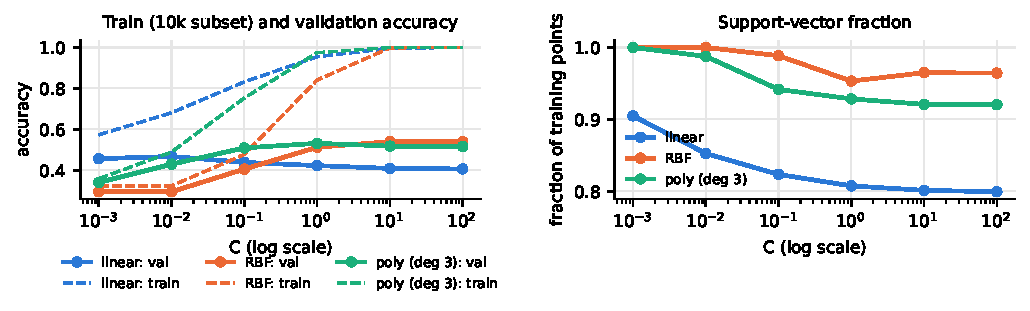
\includegraphics[width=\textwidth]{q4_sweep}
\caption{Q4(a). Left: validation (solid) and train (dashed) accuracy against $C$. Right: support-vector
fraction against $C$.}
\label{fig:q4sweep}
\end{figure*}

\textbf{Under- and overfitting.} Small $C$ means strong regularisation. RBF and polynomial kernels at
$C\le10^{-2}$ underfit badly (train 0.32--0.49, validation close to train) and every training point is a
support vector: with a tiny $C$ all points violate the margin and the solution is close to a weighted vote of
the whole training set. The linear kernel shows the opposite failure. In 1024 dimensions with 10k points it
reaches 100\% train accuracy at $C=100$, but validation falls monotonically after $C=10^{-2}$ (0.467 to 0.406):
the extra flexibility fits the training subset without transferring. The RBF kernel improves up to $C=10$ and
then flattens; once it separates the training set, a larger $C$ no longer changes the solution (same SV
fraction, same validation accuracy). The polynomial kernel peaks at $C=1$ and loses 1.5 points beyond it, a mild
overfit. The support-vector fraction stays at 0.80--1.00 throughout: the classes overlap heavily in this code,
so most points lie on or inside some pairwise margin. Its decrease with $C$ marks the move out of the
underfitting regime, but it does not predict validation accuracy (the linear kernel has the fewest support
vectors and generalises worst).

\textbf{Selection.} RBF with $C=10$ has the best validation accuracy (0.539; $C=100$ ties at 0.539). It was refit
on the same subset and evaluated once on the test set: \textbf{0.528}.

\subsection{(b) Difficult class pairs}
The three pairs with the most test confusions of the selected SVM are cat--dog (392), automobile--truck (341)
and bird--deer (288). For each pair, Fig.~\ref{fig:q4pairs} shows the four training support vectors of each class
closest to that pair's one-vs-one boundary and the eight test images of the two classes with the smallest
$|f|$, where $f$ is the pair decision score (positive = first class).

\begin{figure*}[t]
\centering
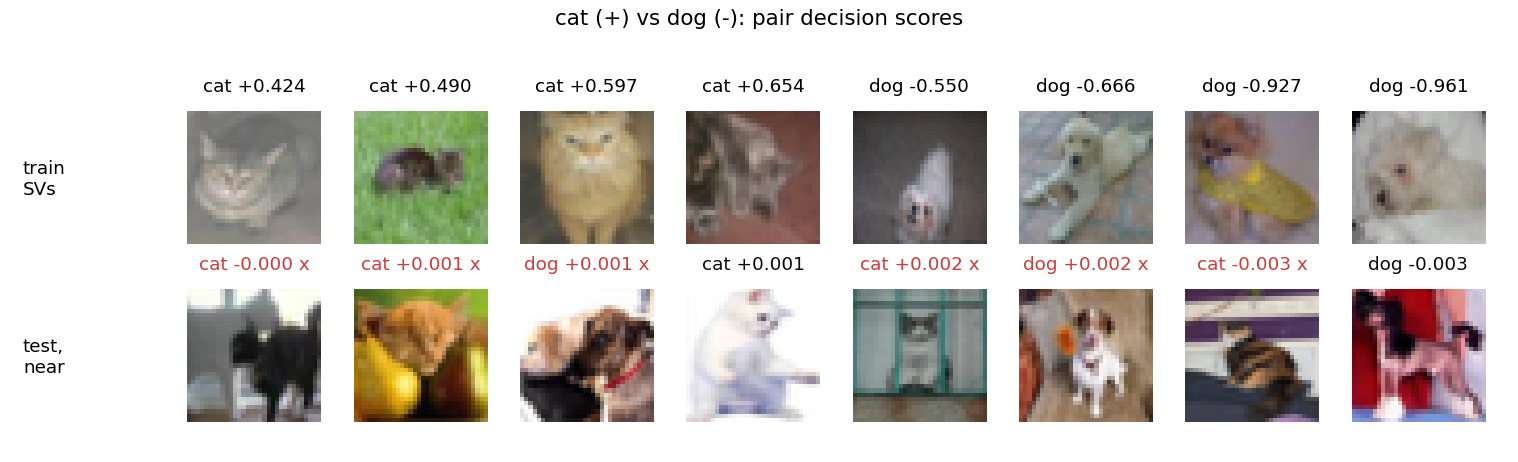
\includegraphics[width=0.82\textwidth]{q4b_pair_cat_dog}\\[-2pt]
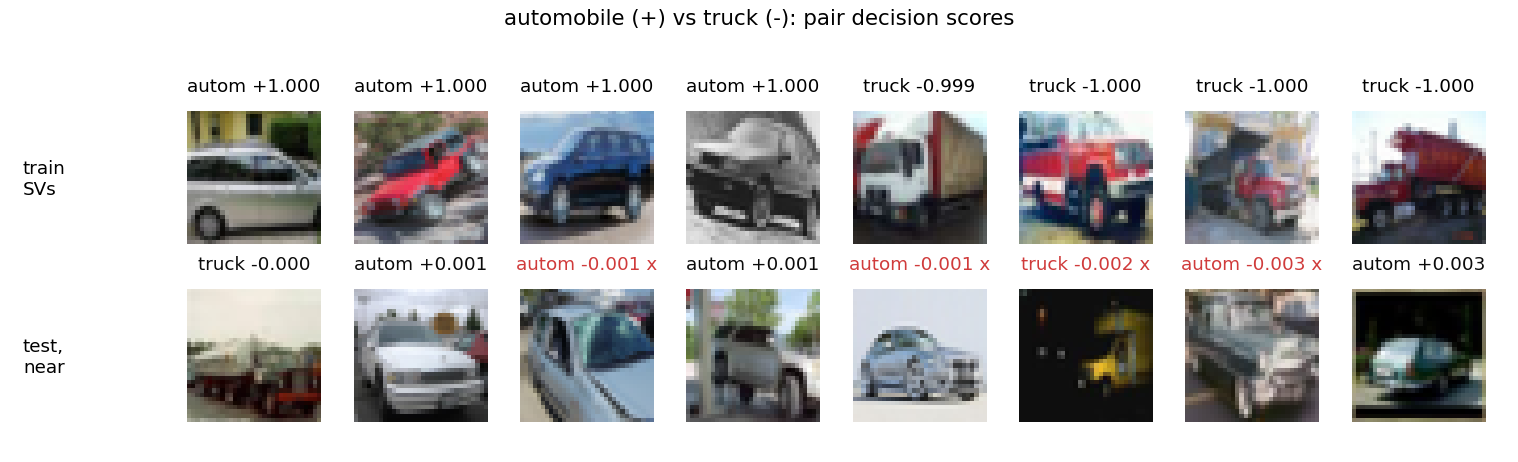
\includegraphics[width=0.82\textwidth]{q4b_pair_automobile_truck}\\[-2pt]
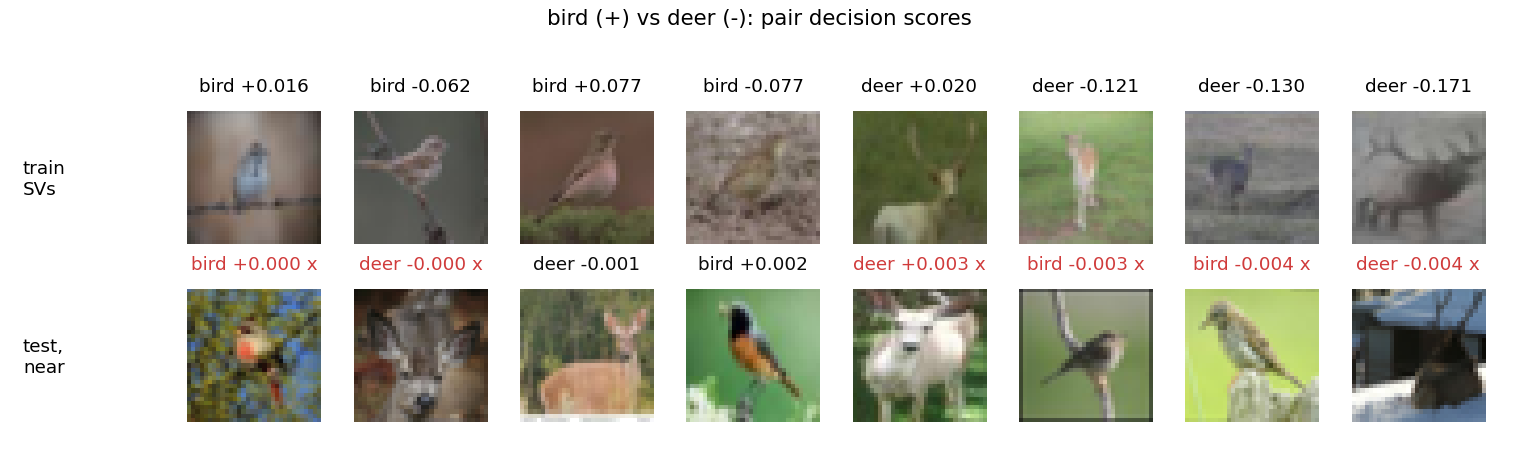
\includegraphics[width=0.82\textwidth]{q4b_pair_bird_deer}
\caption{Q4(b). Per pair, top row: training support vectors closest to the pair boundary; bottom row: test
images nearest the boundary, with the pair decision score. Red ``x'': misclassified by the 10-class SVM.}
\label{fig:q4pairs}
\end{figure*}

\begin{table}[t]
\centering
\small
\resizebox{\columnwidth}{!}{%
\begin{tabular}{@{}lcccc@{}}
\toprule
Pair & Confusions & Pair acc. & Sep.\ ratio & Pair SV frac. \\
\midrule
cat--dog & 392 & 0.634 & 0.015 & 0.95 \\
automobile--truck & 341 & 0.771 & 0.027 & 0.92 \\
bird--deer & 288 & 0.703 & 0.017 & 0.84 \\
\midrule
median of 45 pairs & -- & -- & 0.064 & -- \\
frog--ship (easiest) & 28 & 0.947 & 0.165 & -- \\
\bottomrule
\end{tabular}}
\caption{Q4(b). Test confusions (both directions), accuracy of the pair classifier on the test images of the two
classes, separation ratio (squared distance of class means over mean within-class spread, training codes) and
fraction of the pair's training points that are its support vectors.}
\label{tab:q4pairs}
\end{table}

\textbf{Errors and geometry.} In all three pairs many of the test images nearest the boundary are errors
(6, 4 and 6 of 8). The images explain the geometry. Near the cat--dog boundary are medium-sized furry animals in
the middle of the frame with grey, white or ginger fur; colour, pose and background, which the code encodes
well, do not separate them. The automobile--truck boundary is populated by silver and white vehicles seen from
the side or front, often on plain backgrounds, and dark night images. Bird and deer support vectors are small
brown or grey animals on brown and green natural backgrounds, and they sit deep inside the margin
($|f|<0.2$). Quantitatively (Tab.~\ref{tab:q4pairs}), the class means of these pairs are two to four times closer,
relative to their spread, than for a median pair, and 84--95\% of their training points are support vectors of
the pair classifier, so the boundary has to be supported by nearly the whole pair: the classes overlap instead of
being separated by a gap. Over all 45 pairs the separation ratio and the number of test confusions have a
Spearman correlation of $-0.83$, so the SVM's errors follow the geometry of the representation closely.

\subsection{(c) Clustering the same representation}
\textbf{Method and selection.} $k$-means ($k$-means++, 10 restarts) and diagonal Gaussian mixtures (3 restarts)
with $k\in\{5,10,15,20,30\}$ were fitted on the 45k training codes without labels. The choice used validation
data only: $k$-means with $k=10$ has the highest validation ARI~\cite{hubert1985comparing} (0.062; GMM at most
0.053). NMI was not used for the choice because it keeps increasing with $k$ (0.077 to 0.131). Validation
silhouettes are close to zero or negative for every candidate, a first sign that the code has little cluster
structure. The final model is the one fitted on the training codes; test codes are assigned with it and the test
labels are used only afterwards.

\begin{figure}[t]
\centering
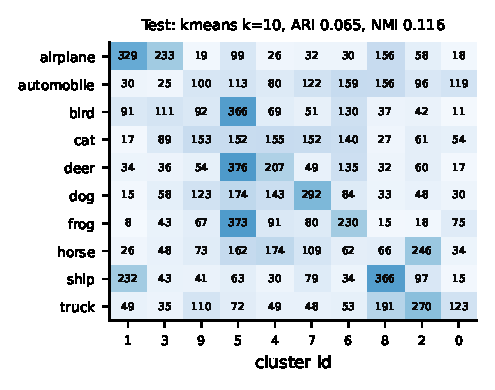
\includegraphics[width=\columnwidth]{q4_contingency}
\caption{Q4(c). Test cluster-to-class contingency table ($k$-means, $k=10$), clusters ordered by majority
class.}
\label{fig:q4cont}
\end{figure}

\textbf{Test result.} ARI 0.065 and NMI 0.116 (Fig.~\ref{fig:q4cont}), against 0.528 accuracy for the SVM. The
clusters follow colour and background more than class: one cluster collects airplanes and ships (329 and 232,
blue sky or water), another birds, deer and frogs (366, 376, 373, green and brown scenery).

\textbf{Where classification and clustering disagree.} The clearest case is \emph{automobile}. For the SVM it is
the easiest class (test recall 0.668, the highest of the ten). For the clustering it is, together with cat, the
least coherent: its largest cluster holds only 15.9\% of the automobile test images, and the row is spread over
all ten clusters (25 to 159 images each). At the pair level, the one-vs-one SVM separates automobile from cat
with 0.905 accuracy on their test images, whereas a vote in which every cluster is labelled with the majority of
the two classes among its members reaches only 0.631, and 85\% of the automobile and cat test images sit in
clusters where both classes make up at least a quarter. The same holds for automobile--horse (0.923 vs 0.658)
and automobile--dog (0.937 vs 0.675). Cars come in every colour and on every background, so colour-driven
clusters break them up, yet the code still contains directions that separate them from animals, and a supervised
RBF SVM finds them. A class can be separable without being compact, and clustering only sees the second
property. No pair goes the other way; the closest is cat--dog, where both are near chance (0.634 vs 0.584).

\section{Reproducibility and conclusion}
\label{sec:repro}
The repository (\repourl, commit \commit) contains all code, the saved split, per-question configurations in the
scripts, the final logs and result files from which every number in this report is read, the figure scripts,
\texttt{requirements.txt} and the exact commands in \texttt{README.md}. Hardware: one RTX 4050 laptop GPU;
SVMs and clustering on the CPU. Seeds are fixed everywhere (242003); GPU kernels are not forced to be
deterministic, so retraining can move results by a few tenths of a point.

Across the four questions one theme repeats: the measurement that looks most natural is often not the one
that answers the question. Final accuracy alone does not tell underfitting from missing priors (Q1a); the final
model hides that structure was learned before memorisation (Q1b); pixel error does not measure usable
information (Q3); and a good classifier on a representation does not imply that the classes form clusters in it
(Q4). The controlled comparisons above are what separate these explanations.


{
\small
\bibliographystyle{ieeenat_fullname}
\bibliography{refs}
}

\end{document}
